\chapter[Fresnel Coefficients][Fresnel Coefficients]{Fresnel Coefficients}\label{ap:FresnelCoefficients}

\section{Background}
%
The Fresnel coefficients, $r^{(\alpha)}_{ij}$ (where $\alpha$ is the polarization), give the ratio of electric field before and after the reflection off a planar interface. The Fresnel coefficients depend on wavelength (through the optical properties), the angle of incidence, and the polarization of light. The polarization (essentially orientation) of light is said to either be $s$ (also called transverse electric, TE, or $\perp$) or $p$ (also called transverse magnetic, TM, or $\parallel$). In some sense, the orientation of the fields is arbitrary and two main conventions exist in the literature for the $p$ polarization. In this work, we will follow the convention of Hecht.\cite{Hecht2017} The main difference is that, for the convention used in this work, $r^{(p)} = - r^{(s)} $ at normal incidence. In the opposing convention, the two quantities are equal. A diagram of the convention used here appears in Fig. \ref{fig:FieldConvention}.

One difference between the present treatment and that of Hecht is that we will not use angles directly when examining angles of incidence. For complex refractive indices, Snell's law predicts complex angles, which I find distasteful. Instead, we will use the in-plane component of the wavevector, $k_{\rho}$, to indicate angles. The main advantage is that $k_{\rho}$ stays constant and real in all media. It may be related to the angle of incidence by $k_{\rho} = (2 \pi /\lambda) \cos{\theta}$. A diagram of the components of the wavevector can be seen in Fig. \ref{fig:FieldConvention}A.

\begin{figure}
\centering
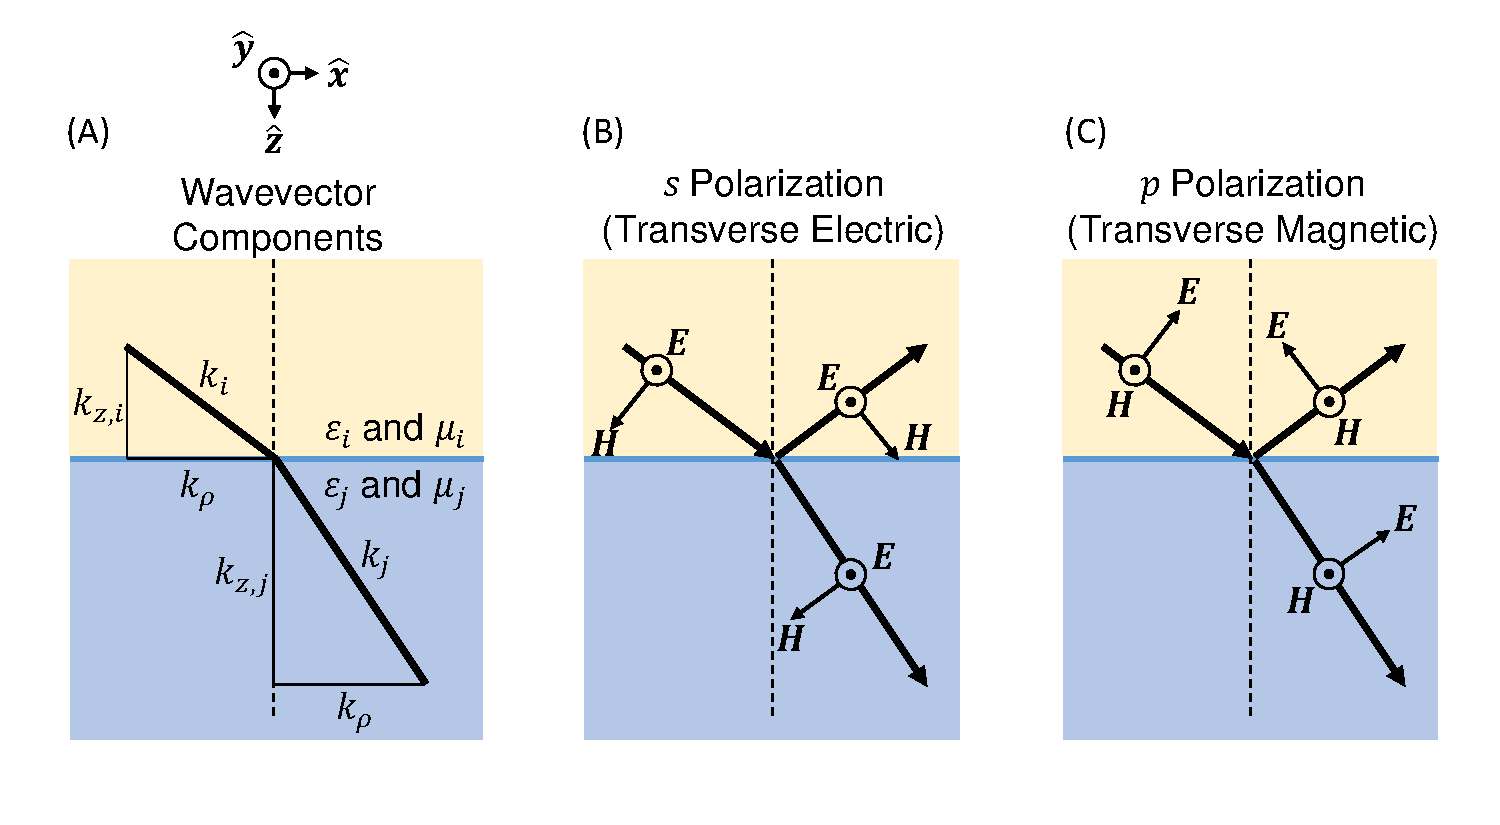
\includegraphics[width=1.0\textwidth]{./Figures/ReflectionConvention.pdf}
\caption{\label{fig:FieldConvention}(A) Diagram of wavevector components and optical properties. (B) Diagram showing orientation of electric and magnetic fields for reflection of $s$ polarization light. (C) Diagram showing orientation of electric and magnetic fields for reflection of $p$ polarization light. }
\end{figure}

\section{Reflection Coefficients} 
%
The Fresnel coefficients between media $i$ and $j$ are given by
%
\begin{subequations}
\begin{align}
r_{i,j}^{(s)} &= \frac{ \frac{k_{z,i}}{\mu_{i}} - \frac{k_{z,j}}{\mu_{j}} }{ \frac{k_{z,i}}{\mu_{i}} + \frac{k_{z,j}}{\mu_{j}} } \\
r_{i,j}^{(p)} &= \frac{ \frac{k_{z,i}}{\varepsilon_{i}} - \frac{k_{z,j}}{\varepsilon_{j}} }{ \frac{k_{z,i}}{\varepsilon_{i}} + \frac{k_{z,j}}{\varepsilon_{j}} }
\end{align}
\end{subequations}

\subsection{Reflectance}
%
Commonly in optics problems, the ratio of electric fields is not a directly useful quantity. Instead, the ratio of electric field intensities is more useful. That ratio is called the reflectance, and is given by
%
\begin{equation}
R_{i,j}^{(\alpha)} = \left| r_{i,j}^{(\alpha)} \right|^{2}
\end{equation}
%
where $\alpha =$ $s$ or $p$.

\subsection{Stratified Media}
%
When a planar medium has multiple planar layers, an effective Fresnel coefficient can be determined. This is typically done using a transfer matrix method\cite{Katsidis2002, Troparevsky2010} or using the Airy formula,\cite{Airy1833, Kaushik1997, Jen2001, Narayanaswamy2013b} which is commonly determined by counting partial wave contributions to reflection. The Airy formula can be used recursively to account for an arbitrary number of layers. It is given by
%
\begin{equation}
\widetilde{r}_{i,i+1}^{(\alpha)} = \frac{r_{i,i+1}^{(\alpha)} + \widetilde{r}_{i+1,i+2}^{(\alpha)} \exp{\left( 2i k_{z,i+1} d_{i+1} \right)} }{ 1 + r_{i,i+1}^{(\alpha)} \widetilde{r}_{i+1,i+2}^{(\alpha)} \exp{\left( 2i k_{z,i+1} d_{i+1} \right)} } 
\end{equation}
%
where $d_{i}$ is the thickness of layer $i$. The recursion is terminated when a semi-infinite half-space is encountered by using a regular Fresnel coefficient in place of the effective one. 